\documentclass[12pt,a4paper,twocolumn]{article}
\usepackage[margin=2cm,columnsep=0.8cm]{geometry} 
\usepackage{setspace}                    
\usepackage{authblk}                      
\usepackage{graphicx}                    
\usepackage{subcaption}                 
\usepackage{float}                       
\usepackage{booktabs}                   
\usepackage{amsmath,amsfonts,amssymb}   
\usepackage{siunitx}                  
\usepackage[round,sort&compress]{natbib}
\usepackage{hyperref}                    
\usepackage{caption}                    
\usepackage{fancyhdr}                   
\usepackage{xcolor}                    
\usepackage{libertine}
\captionsetup{font=small,labelfont=bf}
\pagestyle{fancy}

\fancyhf{}
\fancyhead[L]{\textit{Running Title}}  % Edit the running title (short title)
\fancyhead[R]{\thepage}

% For incoming students, feel free to use your home university here
\title{Full Title of the Article} % Pick your title (you may go creative here)
\author[1]{First Author} % Each author should be listed
\author[2]{Second Author}
\affil[1]{Graz University of Technology, Graz, Austria}
\affil[2]{University of Graz, Graz, Austria}
\date{\today}
\begin{document}
\maketitle

\begin{abstract}
    This report explains how we classify text into facts and opinions. In Stage 1, we cleaned the data and extracted features like part-of-speech tags, sentiment, named entities, and readability. We combined these with TF-IDF vectors and used to train a Logistic Regression model for fact–opinion classification.

    [Stage 2 Abstract Placeholder]
\end{abstract}

\section{Introduction}
\label{sec:intro}
Telling the difference between facts and opinions is an important task in NLP. Our goal is to build a model that can classify text into "fact" or "opinion". 

The project is divided into two stages. Stage 1 focuses on data preprocessing, feature extraction, and training a Logistic Regression classifier. We believe facts and opinions have different structures and emotional tones.

[Stage 2 Intro Placeholder]


\section{Related Work}
Text classification is a common NLP task. Many older methods used handcrafted features and dictionaries to find subjective text~\citep{vaswani2017attention}. For example, sentiment analysis and part-of-speech tags are very useful for finding opinions.

[Stage 2 Related Work Placeholder]

\section{Materials and Methods}
\label{sec:methods}
\subsection{Dataset and Preprocessing (Stage 1)}
We used a dataset with 855 text snippets labeled as "fact" or "opinion". After removing 10 duplicates, we had 845 texts left (437 facts and 408 opinions).

For preprocessing, we changed the text to lowercase, removed punctuation, and lemmatized the words. We removed common English stopwords but kept opinion words like "I", "we", "think", and "suggest".

\subsection{Feature Engineering (Stage 1)}
Next, we extracted several features to help our model:
\begin{itemize}
    \item \textbf{Part-of-Speech (POS):} Using NLTK~\citep{bird2009natural}, we counted nouns, verbs, adjectives, and adverbs. Opinions usually have more adjectives and adverbs.
    \item \textbf{Sentiment:} We used VADER~\citep{hutto2014vader} to score the emotional tone of the text.
    \item \textbf{Named Entities (NER):} We used \textit{spaCy} to find entities like people and places. Facts usually have more entities.
    \item \textbf{Readability:} We calculated the average sentence and word length.
    \item \textbf{Errors and Informality:} We counted spelling mistakes and informal punctuation (like "!!").
    \item \textbf{Knowledge Base:} We counted specific fact and opinion cue words.
\end{itemize}

Finally, the extracted features were combined with TF-IDF vectors and used as input to a Logistic Regression model, which served as our Stage 1 baseline classifier.

\subsection{Stage 2 Methods}
[Stage 2 Methods Placeholder]

\section{Results}
\label{sec:results}
\subsection{Stage 1 Results}
Our feature extraction created a set of inputs for the model. To evaluate its robustness, we performed a 5-fold cross-validation, achieving a mean accuracy of 80.24\% with a standard deviation of 2.58\%. Furthermore, the model's overall performance is summarized in Table~\ref{tab:accuracy}, showing an overall accuracy of 81\%.

\begin{table}[h!]
    \centering
    \caption{Accuracy and F1-Score for Stage 1 Model}
    \label{tab:accuracy}
    \resizebox{\columnwidth}{!}{
    \begin{tabular}{lccc}
        \toprule
         \textbf{Class} & \textbf{Precision} & \textbf{Recall} & \textbf{F1-Score} \\
        \midrule
        Fact & 0.81 & 0.82 & 0.82 \\
        Opinion & 0.80 & 0.80 & 0.80 \\
        \midrule
        \textbf{Overall Accuracy} & \multicolumn{3}{c}{\textbf{0.81}} \\
        \bottomrule
    \end{tabular}
    }
\end{table}

Figure~\ref{fig:confusion_matrix} shows the confusion matrix for our Stage 1 model predictions.

\begin{figure}[h!]
    \centering
    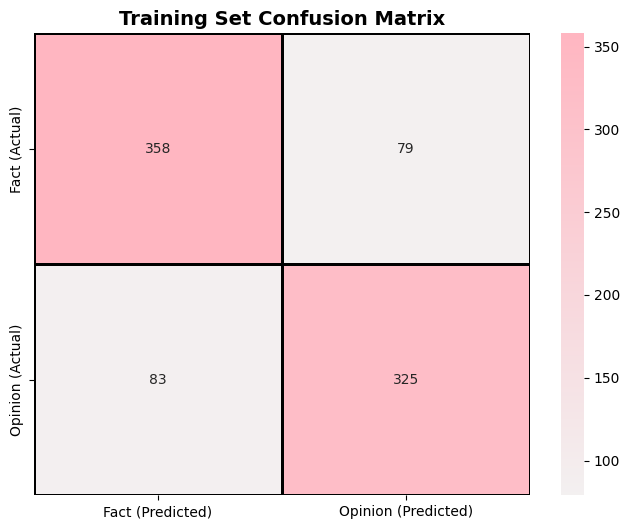
\includegraphics[width=0.8\linewidth]{confusion_matrix.png}
    \caption{Confusion Matrix for Stage 1 Model.}
    \label{fig:confusion_matrix}
\end{figure}

\subsection{Stage 2 Results}
[Stage 2 Results Placeholder]

\section{Discussion}
\label{sec:discussion}
\subsection{Stage 1 Discussion}
The features we extracted showed clear differences between facts and opinions. Opinions had higher sentiment scores and more adjectives, while facts had more named entities. By combining these features with TF-IDF, we created an easy-to-understand baseline model.

\subsection{Stage 2 Discussion}
[Stage 2 Discussion Placeholder]

\section{Conclusion}
\label{sec:conclusion}
In Stage 1, we built a complete data cleaning and feature extraction pipeline. By using POS tags, sentiment scores, and readability metrics, we successfully trained a baseline model to classify facts and opinions.

[Stage 2 Conclusion Placeholder]

Future research could explore using deep learning to further improve results.


% Everything up here counts for the page limit 
\newpage

\section*{Limitations}
One major limitation is that our model only works for the English language. Also, our dataset was relatively small (845 texts), which might make it hard for the model to generalize to completely new topics or very long articles.

\section*{Ethical Considerations}
A potential risk of this work is that a classification model could incorrectly label a true fact as an opinion, which might contribute to misinformation if used automatically in news filtering. To be sustainable, we focused on simple features in Stage 1, which required very little computing power and almost zero carbon footprint compared to training large neural networks.


\section*{Acknowledgments}
We would like to thank our course instructors for providing the dataset and guidance throughout this project.

\section*{Contributions}
% Add here a list of the individual contributions per team member
\begin{table}[h!]
    \centering
    \caption{List of contributions per team member.}
    \label{tab:contributions}
    \begin{tabular}{lp{4cm}}
        \toprule
        \textbf{Team Member} & \textbf{Contribution} \\
        \midrule
        Name            & Did all of the work.             \\
        Another Name    & Did not even care to show up.    \\
        \bottomrule
    \end{tabular}
\end{table}

\bibliographystyle{plainnat}
\bibliography{bibliography}

\appendix

\section{Appendix A - Implementation Details}
The feature extraction pipeline was implemented in Python using the \textit{Pandas} library for data manipulation. \textit{NLTK} was used for tokenization and POS tagging, while \textit{spaCy} was utilized for ultra-fast Named Entity Recognition. The hybrid baseline model was built using the \textit{scikit-learn} Logistic Regression classifier.

\section{Appendix B - Usage of Generative AI}
Generative AI tools were used to assist in structuring this report, debugging Python code for data preprocessing, and summarizing feature distributions. 

[Stage 2 Appendix Placeholder: Partner to add any additional appendix items here].

\end{document}
